%% Nothing to modify here.
%% make sure to include this before anything else

\documentclass[10pt]{beamer}

% packages
\usepackage{color}
\usepackage{listings}
\usepackage{graphicx}
\usepackage{array}

% color definitions
\definecolor{mygreen}{rgb}{0,0.6,0}
\definecolor{mygray}{rgb}{0.5,0.5,0.5}
\definecolor{mymauve}{rgb}{0.58,0,0.82}
\definecolor{php-blue}{HTML}{8892BF}

\setbeamercolor{progress bar}{fg=php-blue}
\setbeamercolor{frametitle}{bg=php-blue}
\setbeamercolor{title separator}{fg=php-blue}
\setbeamercolor{progress bar in section page}{fg=php-blue}
\setbeamercolor{progress bar in head/foot}{fg=php-blue}

% preset-listing options
\lstset{
  backgroundcolor=\color{white},
  % choose the background color;
  % you must add \usepackage{color} or \usepackage{xcolor}
  basicstyle=\footnotesize,
  % the size of the fonts that are used for the code
  breakatwhitespace=false,
  % sets if automatic breaks should only happen at whitespace
  breaklines=true,                 % sets automatic line breaking
  captionpos=b,                    % sets the caption-position to bottom
  commentstyle=\color{mygreen},    % comment style
  % deletekeywords={...},
  % if you want to delete keywords from the given language
  extendedchars=true,
  % lets you use non-ASCII characters;
  % for 8-bits encodings only, does not work with UTF-8
  frame=single,                    % adds a frame around the code
  keepspaces=true,
  % keeps spaces in text,
  % useful for keeping indentation of code
  % (possibly needs columns=flexible)
  keywordstyle=\color{blue},       % keyword style
  % morekeywords={*,...},
  % if you want to add more keywords to the set
  numbers=left,
  % where to put the line-numbers; possible values are (none, left, right)
  numbersep=5pt,
  % how far the line-numbers are from the code
  numberstyle=\tiny\color{mygray},
  % the style that is used for the line-numbers
  rulecolor=\color{black},
  % if not set, the frame-color may be changed on line-breaks
  % within not-black text (e.g. comments (green here))
  stepnumber=1,
  % the step between two line-numbers.
  % If it's 1, each line will be numbered
  stringstyle=\color{mymauve},     % string literal style
  tabsize=4,                       % sets default tabsize to 4 spaces
  title=\lstname
  % show the filename of files included with \lstinputlisting;
  % also try caption instead of title
}

% macro for code inclusion
\newcommand{\includecode}[2][c]{
	\lstinputlisting[caption=#2, style=custom#1]{#2}
}

\usepackage[english]{babel}
% \usepackage[ngerman]{babel}

\usepackage[utf8]{inputenc}
\usetheme{metropolis}

\newcommand{\course}{
	PHP-Kurs
}

\author{
	Alexander Lichter
}

\lstset{
	language = PHP,
	showspaces = false,
	showtabs = false,
	showstringspaces = false
}

% meta-information
\newcommand{\topic}{
	% TODO fill in the actual topic
	PHP-Einführung - Lesson 8 - Composer (Dependency manager) and JSON
}

\title{\topic}
\date{\today}

% the actual document
\begin{document}

\maketitle

\begin{frame}{Content of this lesson}

	\setbeamertemplate{section in toc}[sections numbered]
	\tableofcontents

\end{frame}

\section{Recap}

\begin{frame}{Recap Recap Recap}
%TODO
\end{frame}

\section{Composer}

\begin{frame}{Questions about the installation?}
	Do you have questions concerning the installation of Composer? We have time to go through them now!
\end{frame}

\begin{frame}{Basic usage of composer - Version}
	Alright, we are good to go now! \pause
	Let's start with an easy command: \texttt{composer -v} \pause
	It should show you the version of your installed composer
\end{frame}

\begin{frame}{Basic usage of composer - Init}
	Okay. Let's initialize composer for our project. 
	Each project has it's own composer file and it's own dependencies (obviously) \pause
	
	
	Now go to your project root folder and issue \texttt{composer init} \pause
	You now should walk through the init wizard without problems.
	
	When it you are asked if you want to add your dependencies interactively, write \texttt{no}. Same goes for the dev-dependencies. Now confirm the generation!

\end{frame}

\begin{frame}{Basic usage of composer - Lock and JSON file}
	Congratulations! Your composer file is ready to go! You have a composer.json and a composer.lock file in your project root now. While the composer.json is used for the configuration of composer, the composer.lock saves the currently imported dependencies (with the exact versions).\pause
	
	\textbf{But why do we need a lock file?}\pause
	
	It's great for deploying on production servers, because you get the exact same dependencies as you have on your testing/local environment. Which means: Your production environment is (almost) equal to your local one.
	
	When committing to a VCS \pause (Git, or SVN [but better go for git]), commit both files!
\end{frame}

\begin{frame}{Basic usage of composer - Different dependencies}
	Two slides before, when we initialized our composer setup, I've mentioned \textbf{dependencies} and \textbf{dev-dependencies}. So we have two different dependency "types".. But \textbf{why?} \pause
	
	Dev-dependencies are only those dependencies we need to develop our application. They shouldn't appear on our production server. Things like: Mockup libaries, Testing systems (PHPUnit), Debug tools, and so on. \pause
\end{frame}


\begin{frame}{Basic usage of composer - Require and Install}
	This leads us to the next steps: Setting up dependencies
	This will work with \texttt{composer require[-dev] AUTHOR/PACKAGE [version]}, while require is for "normal" dependencies and require-dev is for dev-dependencies \pause
	
	The version constraint is optional. We'll talk about that in a few minutes! If you don't pass anything, the latest version is used. \pause
	
	If you want to install your dependencies based on your .lock file now (on another PC/Server e.g.), you can use \texttt{composer install [--no-dev]}. Again, --no-dev is used for production and will \textbf{not install} dev-dependencies.
	
\end{frame}

\begin{frame}{Basic usage of composer - Update dependencies}
	Every now and then you may want to \emph{update} your dependencies :D (New features, security stuff and so on). This will work with only \textbf{one command}: \texttt{composer update}\pause
	
	And that's it! Your .lock file is updated too, so you don't need to worry about that.
\end{frame}

\begin{frame}{Basic usage of composer - Versions}
	The cool thing in composer is: You can setup your version constraint by a huge set of rules. Each developer has his own "scheme" about how to provide minor/major/patch/hotfix updates, so this won't be a problem for you too if you setup the versions correctly. \pause
	
	\begin{tabular}{p{2cm} | p{4cm} | p{4cm}}
		Type &  Example & Description \\
		\hline \pause
		Exact & 1.0.2 & Exact version number (and \textbf{only this version}) \pause \\
			\hline \pause
		Range & \textgreater=1.0 \textless1.9 & A simple version range \pause \\
		\hline \pause
		Range (-) & 1.0 - 2.0 & The same as \textgreater=1.0.0 \textless2.1 \pause \\
		\hline \pause
		Wildcard & 1.0.* & Equal to \textgreater=1.0 \textless1.1 \pause \\
		\hline \pause
		Tilde & \textasciitilde1.2.3 & Like \textgreater=1.2.3 \textless1.3.0 \pause \\
		\hline \pause
		Caret & \textasciicircum1.2.3 & Like \textgreater=1.2.3 \textless2.0.0 (ideal for non-breaking) \\
		\hline
	\end{tabular}
\end{frame}

\begin{frame}{Basic usage of composer - Removing dependencies and global installation}
	Removing dependencies is as easy as adding them:
	
	 \texttt{composer remove AUTHOR/PACKAGENAME}\pause
	 
	 
	 Sometimes, you may like to add a dependency globally, and therefore for your whole machine. 
	 
	 \texttt{composer global require AUTHOR/PACKAGENAME}\pause
	 
	 Be aware that you need to add them to your production machine manually then!
\end{frame}

\begin{frame}{Basic usage of composer - Where to find package names}
	Sometimes you may have an idea what packages you need for your applications, but you don't know the name(s)... So, what can we do?\pause
	
	\begin{itemize}
		\item Look up on their git repository \pause
		\item Use \texttt{composer search NAME} \pause
		\item Search on \url{https://packagist.org/}
	\end{itemize}
\end{frame}

\begin{frame}{Basic usage of composer - Autoloading}
	One of the greatest features of composer? It creates an Autoloader for all dependencies!
	You can require the \texttt{vendor/autoload.php} file and you are good to go!\pause
	
	(All dependencies are saved in /vendor. You \emph{must not need} commit this file to your VCS)
\end{frame}


\begin{frame}{Basic usage of composer - Let's require!}
	Okay! For our next topics we need a library called "Collect". It is a \textbf{split} from the Laravel Framework Collection package and will help us to deal with data well.
	
	Let's require it for our project! It's called \textbf{tightenco/collect}
	
\end{frame}

\section{JSON}

\begin{frame}[fragile]{What is JSON}

	JSON stands for JavaScript Object Notation. It's a human-readable data transmission format, that is lightweight and language-independent. Because it is text-only, it is widely used for communicating between browser and server through an API. It can also easily transmit objects, arrays and simple variables.\pause
\begin{lstlisting}
//An JSON object:
{ "name":"Max", "age":21, "city":"San Jose" };
\end{lstlisting}

\end{frame}

\begin{frame}[fragile]{PHP and JSON}
	
	PHP has built-in methods to en- and decode json:
	\begin{lstlisting}
	$object = json_decode('{ "name":"Max", "age":21, "city":"San Jose" }');
	echo $object->name; //Max
	var_dump($object);
	
	echo json_encode($object); //Returns string from above
	\end{lstlisting}
\end{frame}

\begin{frame}[fragile]{DD}
	
	Before we will go through the next tasks, I suggest you another package called \textbf{larapack/dd}. It comes with a function called \texttt{dd()}, which is a "die and dump" aka. debug function. It'll make your life easier when working with arrays. \pause
	
	How to use it:
	\begin{lstlisting}
	$object = json_decode('{ "name":"Max", "age":21, "city":"San Jose" }');
	dd($object);
	\end{lstlisting}
\end{frame}

\begin{frame}[fragile]{Tasks!!!111eleven}
	
	I've set up a little JSON file called tracks.json, that can be found on \url{https://raw.githubusercontent.com/fsr/php-lessons/master/code/tracks.json}
	
	It contains tracks that were downloaded by users of CloudCatcher (\url{www.cloudcatcher.de})\pause
	
	Your first task is to decode the JSON file, without downloading it locally, and printing out the object!\pause
	
	Now, iterate over each element and print out the title! \pause
	
	And finally, reduce your title output to those tracks that have a track number starting with \textbf{165583}
\end{frame}

\begin{frame}[fragile]{Tasks!!!111eleven}
	
	I've set up a little JSON file called tracks.json, that can be found on \url{https://raw.githubusercontent.com/fsr/php-lessons/master/code/tracks.json}
	
	It contains tracks that were downloaded by users of CloudCatcher (\url{www.cloudcatcher.de})\pause
	
	Your first task is to decode the JSON file, without downloading it locally, and printing out the object!\pause
	
	Now, iterate over each element and print out the title! \pause \textbf{BONUS:} Create a array that only contains the titles before!\pause
	
	And finally, reduce your title output to those tracks that have a track number starting with \textbf{165583}
\end{frame}

\section{Collections (next lesson)}

\begin{frame}[plain]
\begin{figure}
	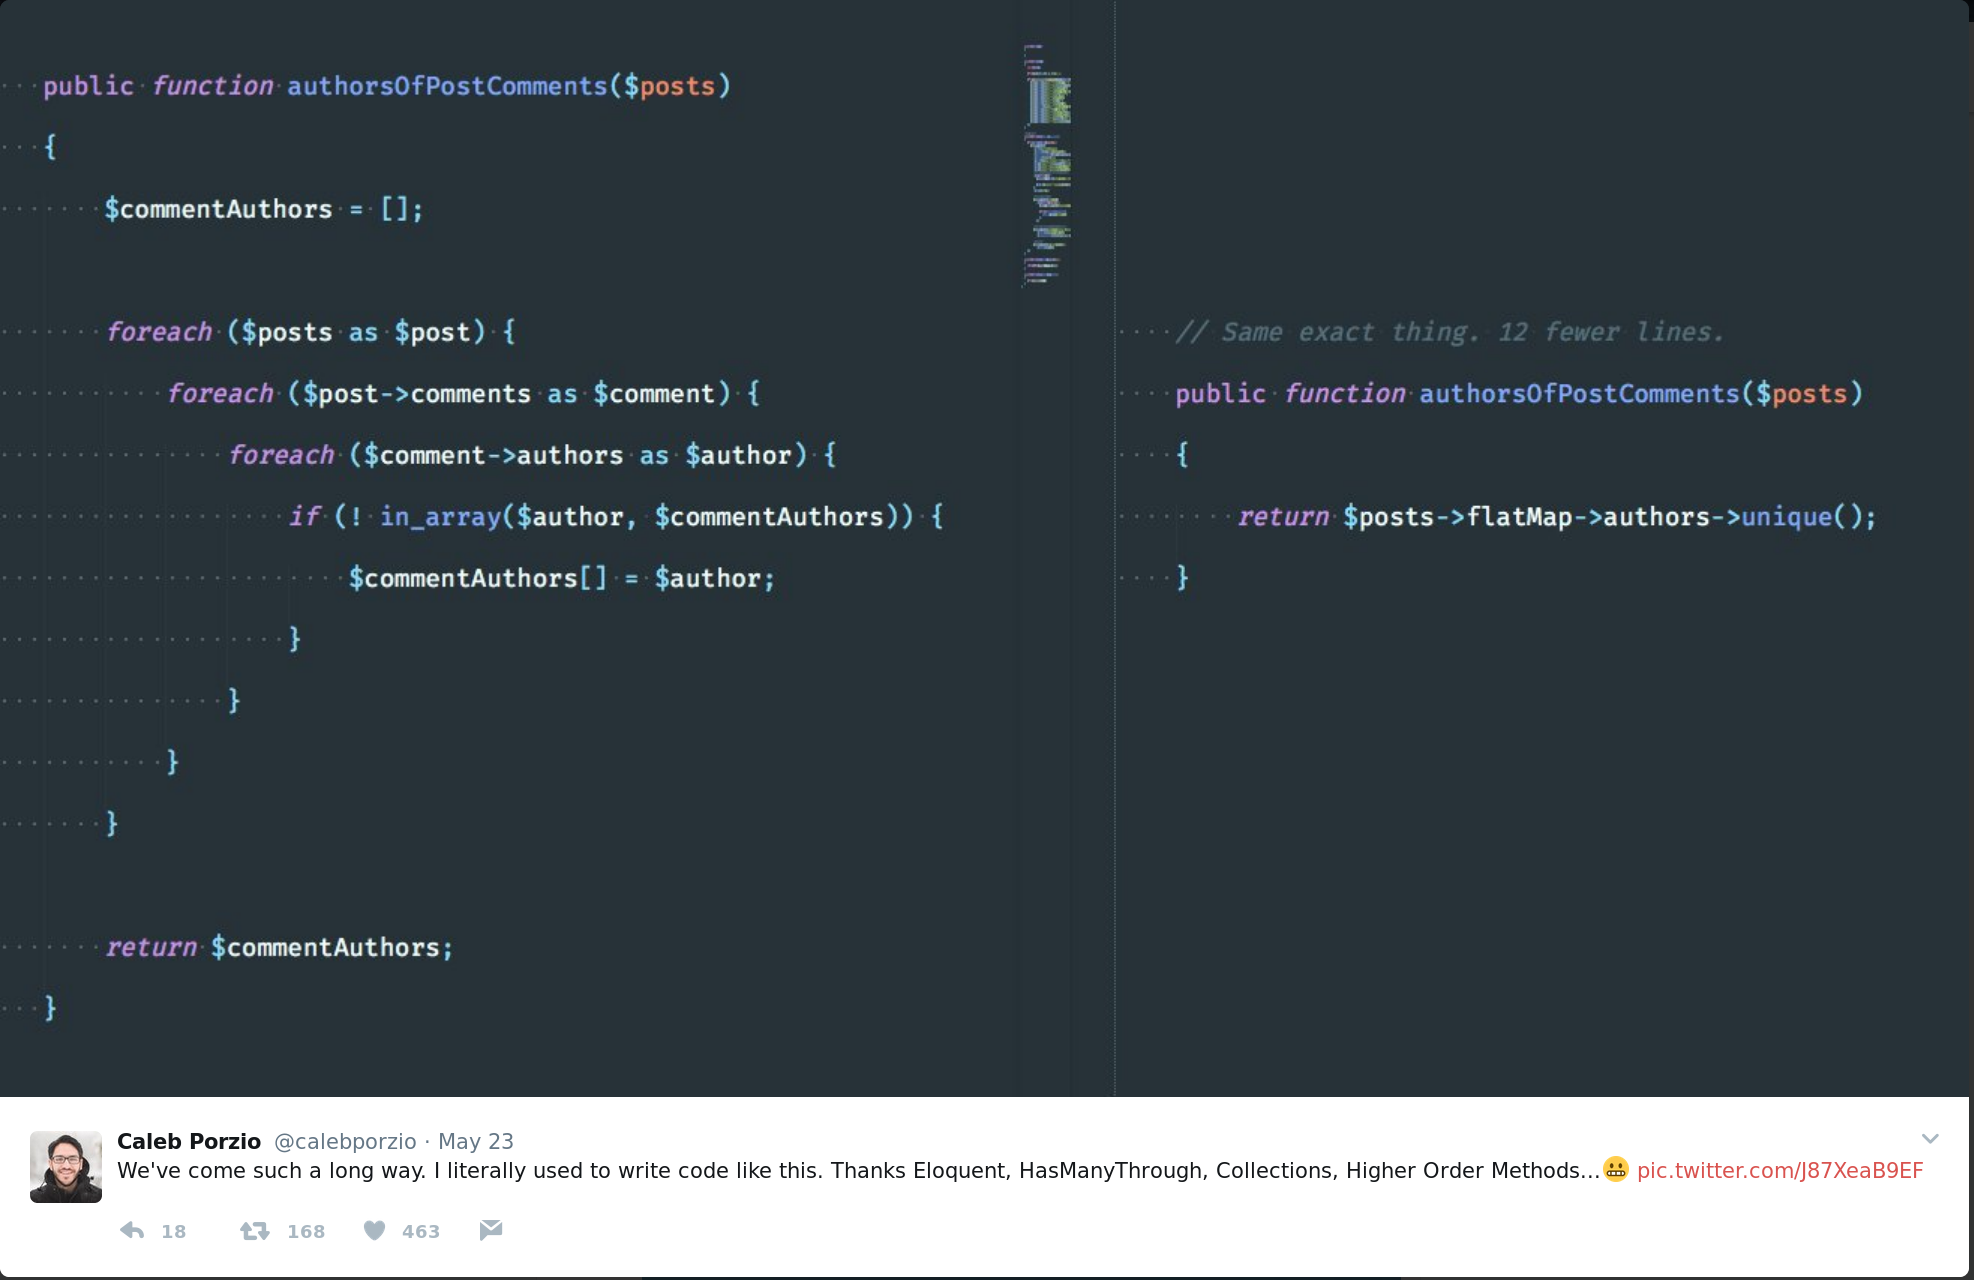
\includegraphics[width=\linewidth]{img/herewecome.png}
\end{figure}
\end{frame}


\end{document}

